\section{Neutrino Oscillations. Theory}

\subsection{Model of Two-Neutrino Oscillations in Vacuum}
Lets consider two neutrinos case as it's described in the chapter 11 of the Griffiths textbook \cite{ref_Griffiths}.\\
Suppose there are only two neutrinos $\nu_e$ and $\nu_{\mu}$. Then true stationary states of the system would be the orthogonal combinations:\\

\begin{center}
$\nu_1=\nu_{\mu}cos\theta-\nu_esin\theta$\\
$\nu_2=\nu_{\mu}sin\theta+\nu_ecos\theta$\\
\end{center}

Then, according to the quantum mechanics,\\
\begin{center}
$\nu_1(t)=\nu_1(0)e^{\frac{-iE_1t}{\hbar}}$, $\nu_2(t)=\nu_2(0)e^{\frac{-iE_2t}{\hbar}}$\\
\end{center}

Suppose, at t=0 there were $\nu_e(0)=1$, $\nu_\mu(0)=0$\\
Then 
\begin{center}
$\nu_1(0)=-sin\theta$, $\nu_2(0)=cos\theta$, $\nu_1(t)=-{sin\theta}e^{\frac{-iE_1t}{\hbar}}$, $\nu_2(t)=-{cos\theta}e^{\frac{-iE_2t}{\hbar}}$\\
\end{center}

Thus, we are getting the system:\\
\begin{center}
$-{sin\theta}e^{-{{iE_1t} \over \hbar}}=\nu_\mu(t)cos\theta-\nu_e(t)sin\theta$,\\
$-{sin\theta}e^{-{{iE_2t} \over \hbar}}=\nu_\mu(t)sin\theta-\nu_e(t)cos\theta$\\
\end{center}

By solving this sytem for $\nu_e$ and $\nu_\mu$, one would get\\
\begin{center}
$P_{\nu_e \rightarrow \nu_\mu}=|\nu_\mu(t)|^2=[{sin2\theta}sin{\frac{(E_1-E_2)t}{2\hbar}}]^2$,\\
$P_{\nu_e \rightarrow \nu_e}=|\nu_e(t)|^2=1-[{sin2\theta}sin{\frac{(E_1-E_2)t}{2\hbar}}]^2$\\
\end{center}

Thus, for freely travelling neutrinos, if $\nu_e$ was emmitted, at any point there is a certain probability to register $\nu_e$ or $\nu_\mu$ and those probablities change with time periodically, by $~[sin(At)]^2$ law. That's why the phenomenon is called the neutrino oscillations.
Suppose momenta $p_1=p_2$. Then using $E^2=p^2+m^2$ and assuming $m_{1,2}<<E_{1,2}$, the probablities will take forms of\\
\begin{center}
$P_{\nu_e \rightarrow \nu_\mu}=|\nu_\mu(t)|^2=[{sin2\theta}sin{\frac{(E_1-E_2)t}{2\hbar}}]^2=[{sin2\theta}sin{\frac{(m_1^2-m_2^2)c^3}{4\hbar{E}}z}]^2$\\  
\end{center}

\subsection{Mechanism of Neutrinos Getting Mass}

\subsection{Three-Neutrino Oscillation}

Three neutrino case is described in the "Long-baseline Neutrino Oscillation Physics" section of the draft Conteptual Design Report (CDR) of the Long Baseline Neutrino Facility (LBNF). For three neutrino case, the oscillations are determined by complex unitary matrix which is called Pontecorvo-Maki-Nakagava-Sakata (PMNS) matrix:\\
\begin{center}
$ \begin{pmatrix} \nu_{e} \\ \nu_{\mu} \\ \nu_{\tau} \\ \end{pmatrix}
 = U_{PMNS}\cdot \begin{pmatrix} \nu_{1} \\ \nu_{2} \\ \nu_{3} \\ \end{pmatrix} = 
 \begin{pmatrix}
  U_{e1} & U_{e2} & U_{e3} \\
  U_{\mu1} & U_{\mu2} & U_{\mu3} \\
  U_{\tau1} & U_{\tau2} & U_{\tau3} \\
 \end{pmatrix}
 \cdot
\begin{pmatrix} \nu_{1} \\ \nu_{2} \\ \nu_{3} \\ \end{pmatrix}$\\
\end{center}
The $U_{PMNS}$ matrix depends on three neutrino mixing angles ($\theta_{12}$, $\theta_{23}$, $\theta_{13}$) and CP-violating phase $\delta_{CP}$. If define $c_{ab}=cos\theta_(ab)$, $s_{ab}=sin\theta_(ab)$, the $U_{PMNS}$ matrix can be splitted into three multipliers, each would be responsible for mixing of one pair of neutrino flavors:\\
\begin{center}
$U_{PMNS} =
 \begin{pmatrix}
  1 & 0 & 0 \\
  0 & c_{23} & s_{23} \\
  0 & -s_{23} & c_{23} \\
 \end{pmatrix}
 \cdot
 \begin{pmatrix}
  c_{13} & 0 & e^{i\delta_{CP}}s_{13} \\
  0 & 1 & 0 \\
  -e^{i\delta_{CP}}s_{13} & 0 & c_{13} \\
 \end{pmatrix}
 \cdot
 \begin{pmatrix}
  c_{12} & s_{12} & 0 \\
  -s_{12} & c_{12} & 0 \\
  0 & 0 & 1 \\
 \end{pmatrix}$ \\
\end{center}
The probability amplitudes of neutrino mixing are defined by parameters of the $U_{PMNS}$ but, analogous to simplified two-neutrino case described above, the differences of squares of neutrino masses also contribute to the probability. There are two independent expressionce for squares of masses differences: ${\Delta}m_{12}^2 = m_1^2-m_2^2$ and ${\Delta}m_{32}^2 = m_3^2-m_2^2$. Mass differences were measured in other neutrino oscillation experiments but the ${\Delta}m_{12}^2$ and ${\Delta}m_{32}^2$ present in the equations evenly and therefore the signs of these expressions were not measured. If the masses order as $m_3 > m_2 > m_1$, it's called normal neutrino mass hierarchy because other fundamental particles orders in a way that later generation particles have higher masses than lower generation particles. If the masses order as $m_1 > m_2 > m_3$ it's called inverted neutrino mass hierarchy. The mixing angles $\theta_{12}$, $\theta_{23}$, $\theta_{13}$ and differences of squared masses $|{\Delta}m_{12}^2|$ and $|{\Delta}m_{32}^2|$ are measured and give $U_{PMNS}$ matrix form of\\
\begin{center}
$|U_{PMNS}| \sim
 \begin{pmatrix}
  0.8 & 0.5 & 0.2 \\ 0.5 & 0.6 & 0.6 \\ 0.2 & 0.6 & 0.8 \\
 \end{pmatrix}$\\
\end{center}
The CP-violating phase $\delta_{CP}$ is unknown.\\*
The analogous matrix for quark mixing, Cabibbo-Kobayashi-Maskawa (CKM) matrix $V_{CKM}$, is much more diagonal:\\*
\begin{center}
$|V_{CKM}| \sim
 \begin{pmatrix}
  1 & 0.2 & 0.004 \\ 0.2 & 1 & 0.04 \\ 0.008 & 0.04 & 1 \\
 \end{pmatrix}$\\
\end{center}
One of the important questions in modern particle physics is why the quark mixing angles are so much smaller than neutrino mixing angles and the other important question is whether there is any relationship between quark and neutrino mixing matrices.\\

The \cite{ref_LBNFdoc_volume-physics} gives the following expression for $\nu_\mu \rightarrow \nu_e$ probability in presence of the Earth matter assuming it has constant density: \\
\begin{center}

\begin{equation}
\label{eq:P_bigFormula}
P(\nu_\mu \rightarrow \nu_e) \simeq P_1 + P_2 + P_3 
\end{equation}

\begin{equation}
\label{eq:P_bigFormula_1}
P_1 = sin^2{\theta_{23}}sin^2{2\theta_{13}}\frac{sin^2(\Delta_{13}-aL)}{(\Delta_{13}-aL)^2}\Delta^2_{31}
\end{equation}

\begin{equation}
\label{eq:P_bigFormula_2}
P_2 = sin2\theta_{23}sin2\theta_{13}sin2\theta_{12}\frac{sin(\Delta_{31}-aL)}{(\Delta_{31}-aL)}\Delta_{31}\frac{sin(aL)}{aL}\Delta_{21}cos(\Delta_{31}+\delta_{CP})
\end{equation}

\begin{equation}
\label{eq:P_bigFormula_3}
P_3 = cos^2\theta_{23}sin^2{2\theta_{12}}\frac{sin^2(aL)}{(aL)^2}\Delta^2_{21}
\end{equation}

where $\Delta_{ij}={\Delta}m^2_{ij}L/4E$, and $a={G_F}{N_e}/sqrt(2)$\\
\end{center}

For $P(\bar{\nu_\mu} \rightarrow \bar{\nu_e})$ one would need to change $\delta_{CP} \rightarrow -\delta_{CP}$ (bacuuse of neutrino-antineutrino assymetry for CP-violationg phase) and $a \rightarrow -a$ (because only electrons present in the Earth, not positrons). The effect of $a \rightarrow -a$ increases with L which means more sensitivity to mass hierarchy for experiments with larger baseline. The planned baseline of the LBNF is 1300 km and it's expected to be enough to determine the neutrino mass hierarchy and also the CP-violation phase.

\begin{figure}
\caption{$P(\nu_\mu \rightarrow \nu_e)$ at a baseline of 1300 km}
\label{fig:LBNF_oscProbability}
\centering
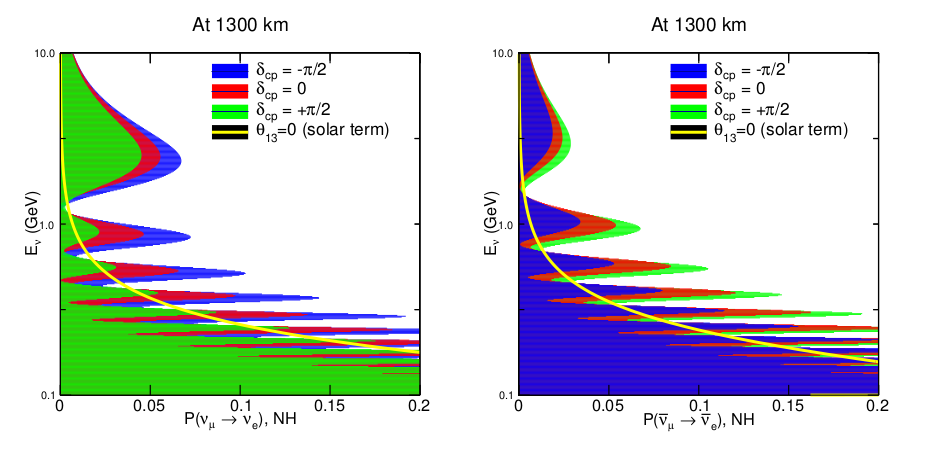
\includegraphics[width=0.98\textwidth, keepaspectratio=true]{figs/LBNF_oscProbability.png}
\\$P(\nu_\mu \rightarrow \nu_e)$ at a baseline of 1300 km, as a function of neutrino energy. Left - neutrinos, right - antineutrinos. Figure is taken from the LBNF CDR draft, volume physics\cite{ref_LBNFdoc_volume-physics}
\end{figure}

The figure \ref{fig:LBNF_oscProbability} shows that magnitude and frequency of oscillations both depend on $\delta_{CP}$ and the differences become more significant for higher oscillation nodes which correspond to lower energies of neutrino/antineutrino. Since changes due to different $\delta_{CP}$s are opposite for neutrinos and antineutrinos, it's important for the experiment to operate both.\\

